%% Submissions for peer-review must enable line-numbering 
%% using the lineno option in the \documentclass command.
%%
%% Camera-ready submissions do not need line numbers, and
%% should have this option removed.
%%
%% Please note that the line numbering option requires
%% version 1.1 or newer of the wlpeerj.cls file, and
%% the corresponding author info requires v1.2

\documentclass[fleqn,10pt,lineno]{wlpeerj}

%%disable for submission
%\linespread{2}

\title{A distribution-based effect size is more reproducible than hypothesis testing when analyzing high throughput sequencing datasets}

\author[1,2]{Andrew D. Fernandes}
\author[2]{Michael Vu}
\author[2]{Lisa-Monique Edward}
\author[2]{Jean M. Macklaim}
\author[2]{Gregory B. Gloor}
\affil[1]{Shield AI Inc., San Diego CA, 92130, United States of America}
\affil[2]{Department of Biochemistry, University of Western Ontario, London, N6A 5C1, Canada}
\corrauthor[5]{G. Gloor}{ggloor@uwo.ca}

% \keywords{Keyword1, Keyword2, Keyword3}

\begin{abstract}
High throughput sequencing is analyzed using a combination of null hypothesis significance testing and ad-hoc cutoffs. This framework is strongly affected by sample size and is known to be irreproducible in underpowered studies, yet no suitable non-parametric alternative has been proposed. Here we present a novel non-parametric standardized  effect size estimate,  $\mathbb{E}$, for high-throughput sequencing datasets. Case studies are shown for modelled data,  transcriptome and  amplicon-sequencing datasets.  The  $\mathbb{E}$ statistic is shown to be more reproducible and robust than p-values and requires sample sizes as small as 5 to  identify  differentially abundant features. Source code and binaries are freely available at: https://bioconductor.org/packages/ALDEx2.html, omicplotR, and  https://github.com/ggloor/distEffect. Datasets can be found at doi://10.6084/m9.figshare.8132216.
\end{abstract}

\begin{document}
\flushbottom
\maketitle
\thispagestyle{empty}


\section*{Introduction}

High throughput sequencing (HTS) datasets for transcriptomics, metagenomics and 16S rRNA gene sequencing are high dimensional and generally  conducted at pilot-scale  sample sizes. Much effort has been spent identifying the best approaches and tools to determine what is `significantly different' between groups \citep{Soneson:2013,Schurch:2016aa}, but the answer seems to depend on the specific dataset and associated model parameters \citep{Thorsen:2016aa,hawinkel2017,Weiss:2017aa}. As commonly conducted, the investigator determines what is `significantly different' using a null hypothesis significance approach and then decides what level of difference is `biologically meaningful' among the significantly different features. Graphically, this approach is  represented by the Volcano plot \citep{Cui:2003aa} where the magnitude of change (difference) is plotted vs the p-value.  

One under-appreciated consequence of pilot-scale research is that false positive features will often have  very low apparent p-values \citep{Halsey:2015aa}. This explains in part why so many observations fail to replicate in larger datasets \citep{Ioannidis:2005aa}. In fact, both p-values and absolute difference are poor predictors of  replication likelihood if the experiment were conducted again \citep{Cumming:2008aa,Halsey:2015aa}. Null-hypothesis significance-based testing methods  also have the property that the number of significant features identified  is affected by the number of samples being compared. This leads to the practice of prioritizing `statistically significant' observations  over biologically  significant differences. 


On the other hand, a standardized effect size addresses the issues of interest to the biologist: ``what is reproducibly different?'' or ``would I identify the same true positive features as different if the experiment were repeated?"  \citep{coe2002s,shinichi:2004,Colquhoun:2014aa,gloor:effect}. Standardized effect size statistics start from the assumption that there is a difference, but that the difference can be arbitrarily close to zero. Unfortunately,  standardized effect size metrics are not routinely used when analyzing HTS datasets. One potential barrier  is that parametric effect size statistics may not be suitable for  HTS datasets because the data may not fit a Gaussian distribution.  

The most widely used standardized effect size is Cohen's d, which is a parametric standardized effect size for the difference between the means of two groups. The general formulation is given in Equation~\ref{eq:cohen},
\begin{equation}
\mathrm{Cohen's~d} = \frac{\mathrm{mean}(a)- \mathrm{mean}(b)}{\sigma_{a,b}}
\label{eq:cohen}
\end{equation}
 and is  a Z score when measured in a Normal distribution. Cohen's d measures the difference between the means of the two distributions divided by the pooled standard deviation, denoted as \(\sigma_{a,b}\). However, this metric depends upon the data being relatively Normal, which cannot be guaranteed for HTS data as seen in Figure \ref{fig:dist}. 

The purpose of this report is to show that  we  can characterize the difference between distributions in a non-parametric manner without resorting to either summarizing the data prematurely or resorting to a rank-based approach, both of which  discard much information. We introduce, $\mathbb{E}$,  a simple-to-calculate non-parametric standardized effect size statistic calculated on distributions directly. This measure is implemented in the ALDEx2, and CoDaSeq R packages.  The $\mathbb{E}$ statistic has been used in both meta-transcriptome and microbiome studies, for example see \citep{macklaim:2013, bian:2017}, and has been shown to give remarkably reproducible results even with extremely small sample sizes \citep{nelson:2015vaginal}.   The $\mathbb{E}$ metric has a near monotonic relationship with p-values, but has the advantage of being relatively stable between sample sizes. However, it is unknown how  $\mathbb{E}$  compares with parametric effect size estimates, how many samples are required, and its sensitivity and specificity characteristics. 

\section*{Methods}

\subsection*{Calculating $\mathbb{E}$}
High throughput sequencing (HTS) platforms such as Illumina output thousands to billions of `reads', short nucleotide sequences that are derived from a DNA or RNA molecule in the sequencing `library'. The library is a subset of the nucleic acid molecules that have been collected from an environment and made compatible with a particular HTS platform. The HTS instruments deliver these reads as integer `counts' per genomic feature---gene, location, etc \citep{lovell2020counts}. However, the counts are actually a single proxy for the probability of observing the particular read in a sample under a repeated sampling model. This is clear since technical replicates of the same library return different counts\citep{Marioni:2008}, and the difference between technical replicates is consistent with multivariate Poisson sampling \citep{fernandes:2013, gloorAJS:2016}. The probability estimate is delivered by the instrument as an integer representation of the probability multiplied by the number of reads  \citep{fernandes:2013, gloorAJS:2016}. Thus, the data returned by HTS are a type of count compositional data, where only the relationships between the features have meaning \citep{aitchison:1986, Lovell:2015, fernandes:2014, gloorFrontiers:2017, Kaul:2017aa, Quinn:2019aa}. 

The ALDEx2 tool uses a combination of probabilistic modelling and compositional data analysis to determine the features that are different between groups where that difference is insensitive to random sampling. Technical replicate variance estimation and conversion of the count data to probabilities is accomplished by Monte-Carlo sampling from the Dirichlet distribution \citep{fernandes:2013, gloorAJS:2016}, which is conveniently also the conjugate prior for the multivariate Poisson process. The differences between features is linearized by applying a log-ratio transformation to the Dirichlet Monte-Carlo realizations and analyzed according to the rules of compositional data analysis \citep{aitchison:1986,fernandes:2013,Tsilimigras:2016aa,gloorFrontiers:2017}. In effect, ALDEx2 linearizes the differences between the features in proportional data, allowing various standard stasticial tests to validly be performed.

The `Group Distribution' panel in Figure 1 shows the distribution for a gene in a highly replicated and curated RNA-seq experiment  \citep{Schurch:2016aa} with the expression of the gene in the WT and knockout conditions  shown by the two density distributions. An Anderson-Darling test indicates that a Normal distribution is a poor fit for both distributions ($p < 1e-4$). Consequently, standard effect size measures that depend on summary statistics that assume a Normal distribution are expected to perform poorly and the non-parametric method described here is to be preferred. 

\begin{figure}[t!]
\centerline{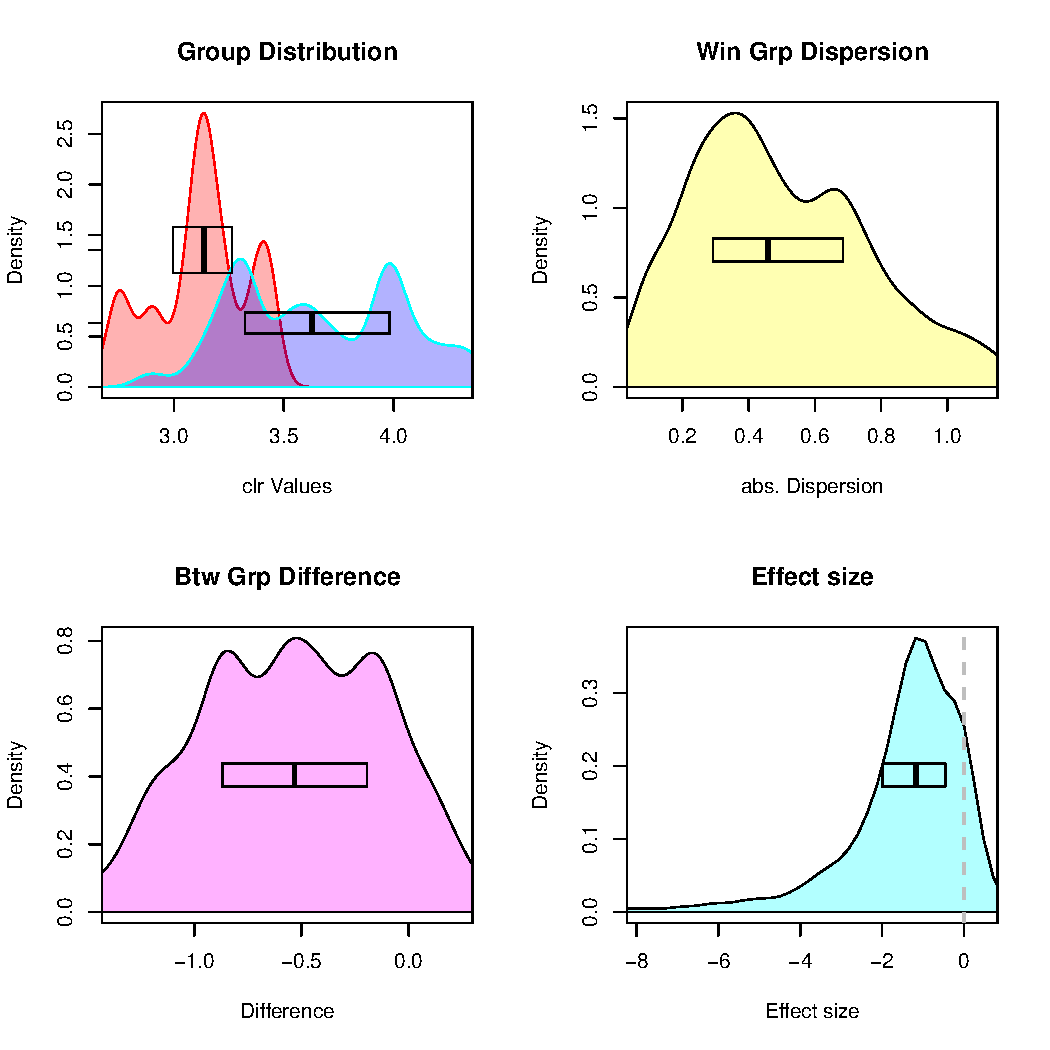
\includegraphics[scale=0.50]{YDR171W_dist.pdf}}
\caption{The density of read counts may not follow a Normal  distribution. The `Group Distribution' panel in the top left shows the density of the clr-transformed read counts in the two groups of a highly replicated RNA-seq experiment conduced in \emph{S. cerevisiae} \citep{Schurch:2016aa} for the gene YDR171W. We can see that the distributions are partially overlapping and are strongly multimodal. The `Win Grp Dispersion' shows the density of the within group dispersion of the two groups calculated as outlined in equation  \ref{eq:disp}. The`Btw Grp Difference' shows the density of the between group difference calculated as outlined in  equation \ref{eq:diff}. The `Effect size' shows the density of the effect size calculated as in equation  \ref{eq:ff}. The dashed vertical line in this final panel shows an effect size of 0, and approximately 10\% of the effect size distribution crosses this threshold for this gene. The proportion of the effect size distribution that crosses an effect of 0 is known as the `overlap' measure. For each distribution the median and interquartile range are shown as the thick vertical line and the enclosing box. This plot was generated from the `aldex.plotFeature()' command.}
\label{fig:dist}
\end{figure}
	
We will use the distributions for the gene YDR171W in Figure \ref{fig:dist} as an example. Starting with two vectors $\vec{a}$ and $\vec{b}$  that correspond to the log-ratio transformed Dirichlet Monte-Carlo realizations of a feature in two groups, we need a method to determine the standardized effect size;  that is, the difference between groups relative to an estimate of within-group dispersion. Since these posterior distributions can have heavy tails, may be multimodal, and may be skewed, any useful statistic should be insensitive to even extreme non-Normality, and  provide sensible answers even if the posterior  distributions are  Cauchy in one or both groups \citep{fernandes:2013}. Below and in the Supplement we define the properties of the approach used.

We can define a non-parametric  \emph{difference} vector  in Equation~(\ref{eq:diff}) as the signed difference between the two groups
\begin{equation}
\vec{\mathit{diff}} = \vec{a} - \vec{b},
\label{eq:diff}\vspace*{-10pt}
\end{equation}
with the distribution of the vector  shown in Figure 1 `Btw Group Difference'.  We can further define a non-parametric  \emph{dispersion} vector as in Equation~(\ref{eq:disp}), where the notation $\boldsymbol{\rho}\vec{a}$ indicates one or more random permutations of the vector
\begin{equation}
\vec{\mathit{disp}} = max \{ \lvert \vec{a} - \boldsymbol{\rho} \vec{a}  \rvert ,\lvert \vec{b} -\boldsymbol{\rho} \vec{b} \rvert \},
\label{eq:disp}\vspace*{-10pt}
\end{equation}
with the distribution shown in Figure 1 `Win Group Dispersion'. Finally, we can define an \emph{effect} vector as in Equation~(\ref{eq:ff}) that is the element-wise ratio of these two vectors 
\begin{equation}
\vec{\mathit{eff}} = \frac{\vec{diff}}{\vec{disp}},
\label{eq:ff}\vspace*{0pt}
\end{equation}

with the distribution of the effect vector shown in Figure 1 `Effect size'.

Taking the median of $\vec{\mathit{diff}}, \vec{\mathit{disp}}$ and $\vec{\mathit{eff}}$ returns a robust estimate of the central tendency of these statistics MSD (median signed difference), MMAD (median of the maximum absolute deviation), and $\mathbb{E}$), and these are the `diff.btw', `diff.win' and `effect' statistics reported by ALDEx2. The median and interquartile range of these summary statistics for each distribution is shown in Figure \ref{fig:dist}. The MSD is  very similar to the difference between the means or the difference between medians in a Normal distribution as shown in Supplementary Figure  1. The MMAD metric is novel and the Supplement shows it has a Gaussian efficiency of 52\%, a breakdown point of 20\% (Supplementary Figure 2), and is 1.42 times the size of the standard deviation on a Normal distribution. The $\mathbb{E}$ statistic is a standardized effect size and is approximately 0.7 of Cohen's d when comparing the difference between two Normal distributions.   Below and in Supplementary Figure 3 we show that this metric returns sensible values even with non-Normal distributions.


We used  simple simulated datasets to determine baseline characteristics in a number of different distributions. Then we use the data  from a highly replicated RNA-seq experiment \citep{Schurch:2016aa} or from a large 16S rRNA gene sequencing study  \citep{bian:2017} and examined 100 random subsets of the data with between 2 and 20 samples in each group. For each random subset we collected the set of features that were called as differentially abundant at thresholds of $\mathbb{E} \ge 1$, or with an expected Benjamini-Hochburg adjusted p-value of $\le 0.1$ calculated using either the parametric Welch's t-test, or the non-parametric Wilcoxon test in the ALDEx2 R package. These are output as `we.eBH' and 'wi.eBH' by the ALDEx2 tool. These were compared to a `truth' set determined by identifying those features that were identified in all of 100 independent tests of the full dataset with outliers removed using the same tests and cutoffs. Note that this is simply a measure of consistency and is congruent with the approach taken in \citep{Schurch:2016aa}. We also examined subsets of these datasets where the subsets were taken from the same group. This allowed us to characterize the properties of $\mathbb{E}$ when no difference between groups was expected.

\enlargethispage{6pt}


\section*{Results and Discussion}

The motivation for this work is to identify what features are reliably different even with the small sample sizes prevalent in high throughput sequencing experiments. Measuring differential abundance in high throughput sequencing datasets is difficult for a variety of reasons. First, almost all experiments are underpowered. Second, the true distribution of the data and the ground truth of the data are both unknown. Third, when sample sizes are large, almost all features are identified as `significantly different' by null hypothesis significance testing frameworks. This latter reason is why ensuring that the feature is below a p-value threshold (or below a q, or false discovery rate,  threshold) and be above a minimum difference threshold is common guidance \citep{Schurch:2016aa}. Graphically, these cutoffs are represented by the volcano plot \citep{Cui:2003aa}. 

We began by examining the behaviour of the $\mathbb{E}$ metric and its constituent statistics. Supplementary Figure 1 shows that the difference between distributions  measure is essentially as efficient and stable a measure of location as is the difference between means. When comparing measures of scale, Supplementary Figure 2 shows that the breakdown point for the MMAD is 20\% and the efficiency is approximately 52\% of the standard deviation in a Normal distribution. Thus, the MMAD is reasonably efficient, and much less prone to contamination than is the standard deviation. Simulation shows that the MMAD is approximately 1.418 larger than the standard deviation for a Normal distribution. Taken together, $\mathbb{E}$  is approximately  0.705 the size of Cohen's d in a Normal distribution, but $\mathbb{E}$ returns sensible estimates even for non-Normal distributions such as $\beta$ and Cauchy distributions. 

The remaining data and figures were generated from two real datasets. The `yeast' dataset is derived from a highly replicated RNA-seq dataset generated by \citep{Schurch:2016aa}, and the `16S' dataset is derived from a large scale cross-sectional survey of the microbiome of healthy chinese volunteers \citep{bian:2017}. Generically the genes or operational taxonomic units that compose the sequence bins will be referred to as 'features'. These two datasets are polar opposites in many ways, with the yeast dataset having very few 0-count features and low variance within groups, and the 16S dataset being very sparse and having high variance within groups. These two datasets are used to investigate the relationships between three measurable summary statistics of the distributions the difference between groups, the effect size and the overlap, and how these values can be used to identify reproducibly different features in high throughput sequencing datasets.

Figure \ref{fig:null}:A shows the relationship between $\mathbb{E}$ and p-values for the 6349 genes in the yeast dataset. We can see that there is very good correspondence such that features with very high effect sizes have very low adjusted p-values. This is in line with the expected relationship between effect sizes and p-values, and provides additional confidence that $\mathbb{E}$ is an appropriate metric for effect size. However, note that the non-parametric Wilcoxon test adjusted p-values (in blue) have far fewer outliers on this plot than do the parametric Welch's t-test adjusted p-values (in red). We conclude that the majority of features likely have distributions that do not deviate too much from the Normality assumption of the parametric test, but that  a significant minority of features have enough deviation to affect the calculated p-value. These outliers could contribute to both false positive and false negative identifications when using a parametric null hypothesis testing approach.

\begin{figure}[tpb]
\centerline{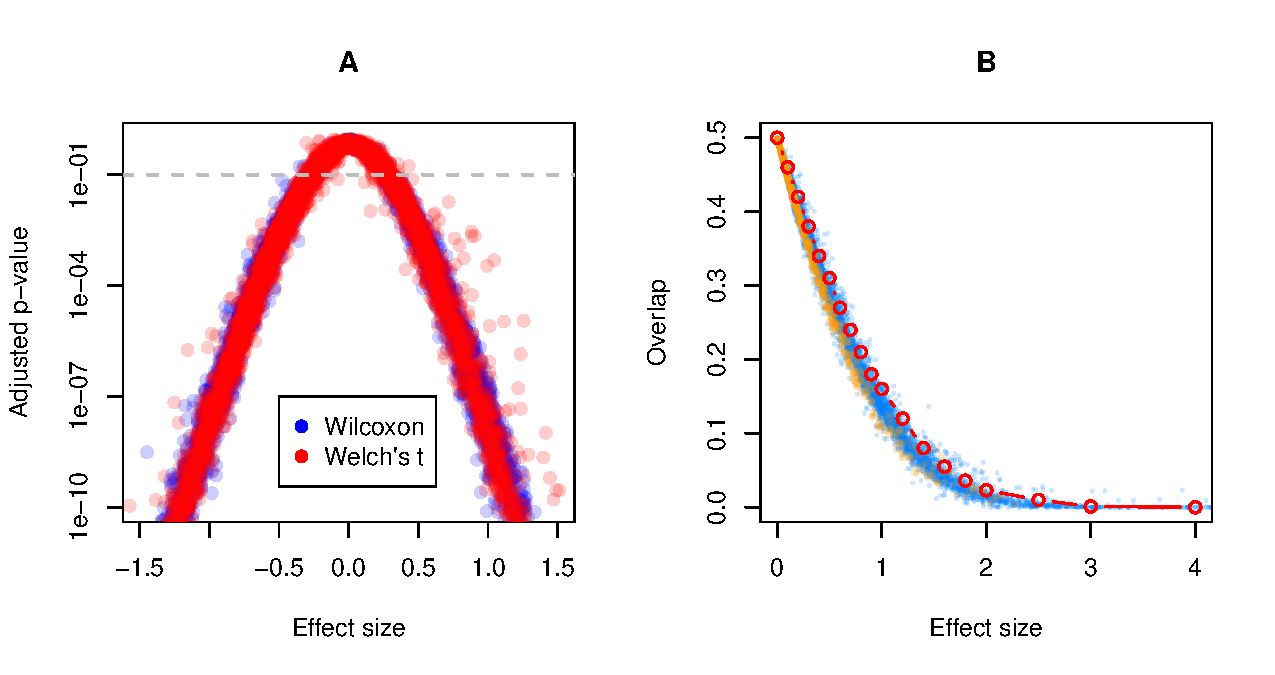
\includegraphics[scale=0.5]{null-effect.pdf}}
\caption{Distributional properties of $\mathbb{E}$. Panel A shows the relationship between  $\mathbb{E}$ and Benjamini-Hochberg adjusted p-values calculated by either a non-parametric Wilcoxon test (blue points), or a parametric Welch's t-test  (red points), where each point represents one of the genes in the yeast transcriptome dataset. The y axis has been truncated to highlight the p-values greater than 1e-10, and the dashed grey line shows the location of a false positive threshold of 0.1. Panel B shows the relationship between  $\mathbb{E}$ and the overlap measure in the yeast dataset (blue points) and the 16S dataset (orange points). Overlaid in red is the expected relationship for a Z-score in a Normal distribution. }
\label{fig:null}
\end{figure}

We next focused on the characteristics of false positive features in the two datasets and  examined the relationship between  the $\mathbb{E}$ and the overlap metrics in both the yeast and 16S datasets. Recall from Figure \ref{fig:dist} that all values are calculated from the distributions and not inferred from summary statistics. The overlap  is the proportion of the a $\mathbb{E}$ distribution where the tail overlaps 0. In a Normal distribution, Cohen's d is exactly equivalent to a Z score, and we can determine the proportion of the tail distribution that corresponds to any Z score (effect size). This relationship is plotted in Figure \ref{fig:null}:B and we can see that the non-parametric $\mathbb{E}$  and overlap metrics correspond very well to the expected relationship for a Z score and tail area in a Normal distribution. On this graph, an overlap of 0.1 corresponds to $ \mathbb{E} \sim 1.2$. 

Next, we  examined the proportion of features that were identified as being false positives as a function of per-group sample size if there was no difference between groups. For this, we generated 100 random instances from both datasets with the samples draws from only one group and the per-group sample size varying from 2 to 20. We calculated the proportion of  all features in the dataset that  had a greater than 2-fold difference; or an overlap less than 0.1;  or that had $\mathbb{E}$ values greater than 0.5, 1, or 2; or that had the intersect of the difference $>1$, overlap $<0.1$ and $\mathbb{E}$ greater than 1. This was plotted relative to the per-group sample size in Fig \ref{fig:fp}:A. A number of observations can be made. First, it is apparent that there is a strong linear relationship between the proportion of features that are identified as false positive and the sample size for all the metrics. Second, a smaller number of samples was needed to ensure no false positive features were identified as the effect size increased; at the extreme an effect size of 2 would be sufficient to exclude FP features with as few as 5 samples per group. Third, difference was a poor measure by which to exclude FP features, being worse as a measure in the highly variable  16S dataset. Fourth, the effect size was highly reproducible as a measure to exclude FP features having almost the same characteristics in both datasets. The overlap measure was also highly reproducible, but this is a trivial finding since Figure \ref{fig:null} shows that effect size and overlap are highly correlated. Fifth, combining the three measures was able to exclude FP features better than was any single metric. However, the triple measure of effect, overlap and difference did not give the same result in the two datasets. In the low variance yeast dataset the triple measure was, if anything, it was even more specific than was doubling  the effect size. In contrast, the triple measure was only slightly more specific in the high variance dataset than were the single measures of $\mathbb{E}$ or overlap.

\begin{figure}[tpb]
\centerline{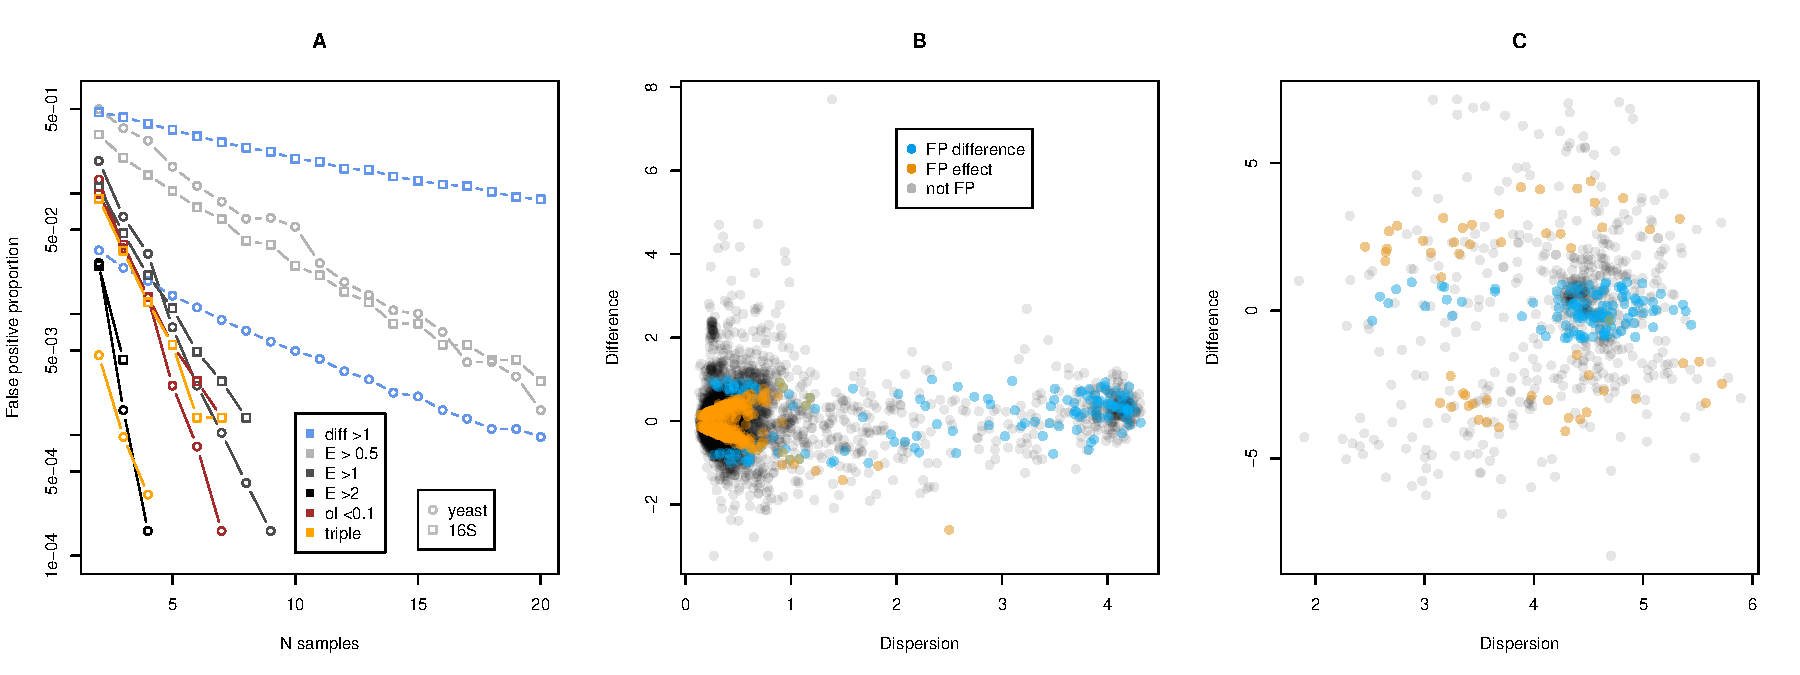
\includegraphics[scale=0.5]{FP-plots.pdf}}
\caption{Characteristics of false positive features using $\mathbb{E}$. Panel A plots per-group sample size and the FP rate of  difference, and the median values when applied to a samples drawn at random from the same group. Also shown is the combination of these three metrics into one metric that is the overlap between the three (triple). Panel B shows an effect plot \citep{gloor:effect} of the whole yeast transcriptome dataset in grey points, with the false positive features identified by either difference between groups (blue) or $\mathbb{E}$ (orange)  identified from a random subset of 5 samples from each group. Panel C shows the same analysis on the 16S rRNA gene sequencing dataset. The false positive features identified by each approach are restricted to features with quite separate characteristics of difference and dispersion.}
\label{fig:fp}
\end{figure}

We used effect plots \citep{gloor:effect} to identify why the triple measure was more specific in the yeast dataset than in the 16S dataset and the results are shown in Figure \ref{fig:fp} panels B and C. Here we overplotted the FP features found when an example dataset of 5 in each group was compared to the TP features found when the full dataset was examined and applying the dual cutoffs of both difference and $\mathbb{E} > 1$.  In the yeast dataset, the FP $\mathbb{E}$ features have very low dispersion (variance) and  very low difference, while the features identified as FP when only difference was used tended to have either very high or very low dispersion. In the 16S dataset, essentially all the features have very high dispersion. Here we found that the FP features identified by  $\mathbb{E}$ have a large between group difference, and the FP features identified only by difference tend to have low difference between groups. This mirrors the observation seen in the yeast dataset. These observations explain why using both $\mathbb{E}$ and difference in combination are  more discriminatory than either alone, as they tend to identify different sets of FP features.


With this  information, we can  determine the sensitivity and specificity of identifying TP and FP features in the example datasets when comparing two groups. In the yeast dataset, the edgeR tool identified over 4600 out of 6349 genes as `significant'  (Benjamini-Hochberg adjusted p-value $< 0.05$) when all samples were included using either the glm or exact test modes (Supplementary Table 1).  Other widely used tools gave similar results \citep{Schurch:2016aa}. The null hypthesis testing framework in ALDEx2 also returned at least 4300 genes in the same dataset. Thus, identifying such a large proportion of genes as differentially abundant indicates that statistical significance is not informative for this type of experiment. Schurch et al. (and others) recommend adding a secondary threshold such as a fold-change cutoff to identify genes of interest for follow-up analyses \citep{Cui:2003aa,Schurch:2016aa}. When sample sizes are sufficiently large, we would expect that the fold-change cutoff itself would be the primary determinant of difference; however, this approach would not include either the biological variance or the uncertainty of measurement in the analysis. Furthermore,  the difference metric is not sufficient to exclude FP features and this is especially relevant for features with large dispersion.


\begin{figure}[tpb]
\centerline{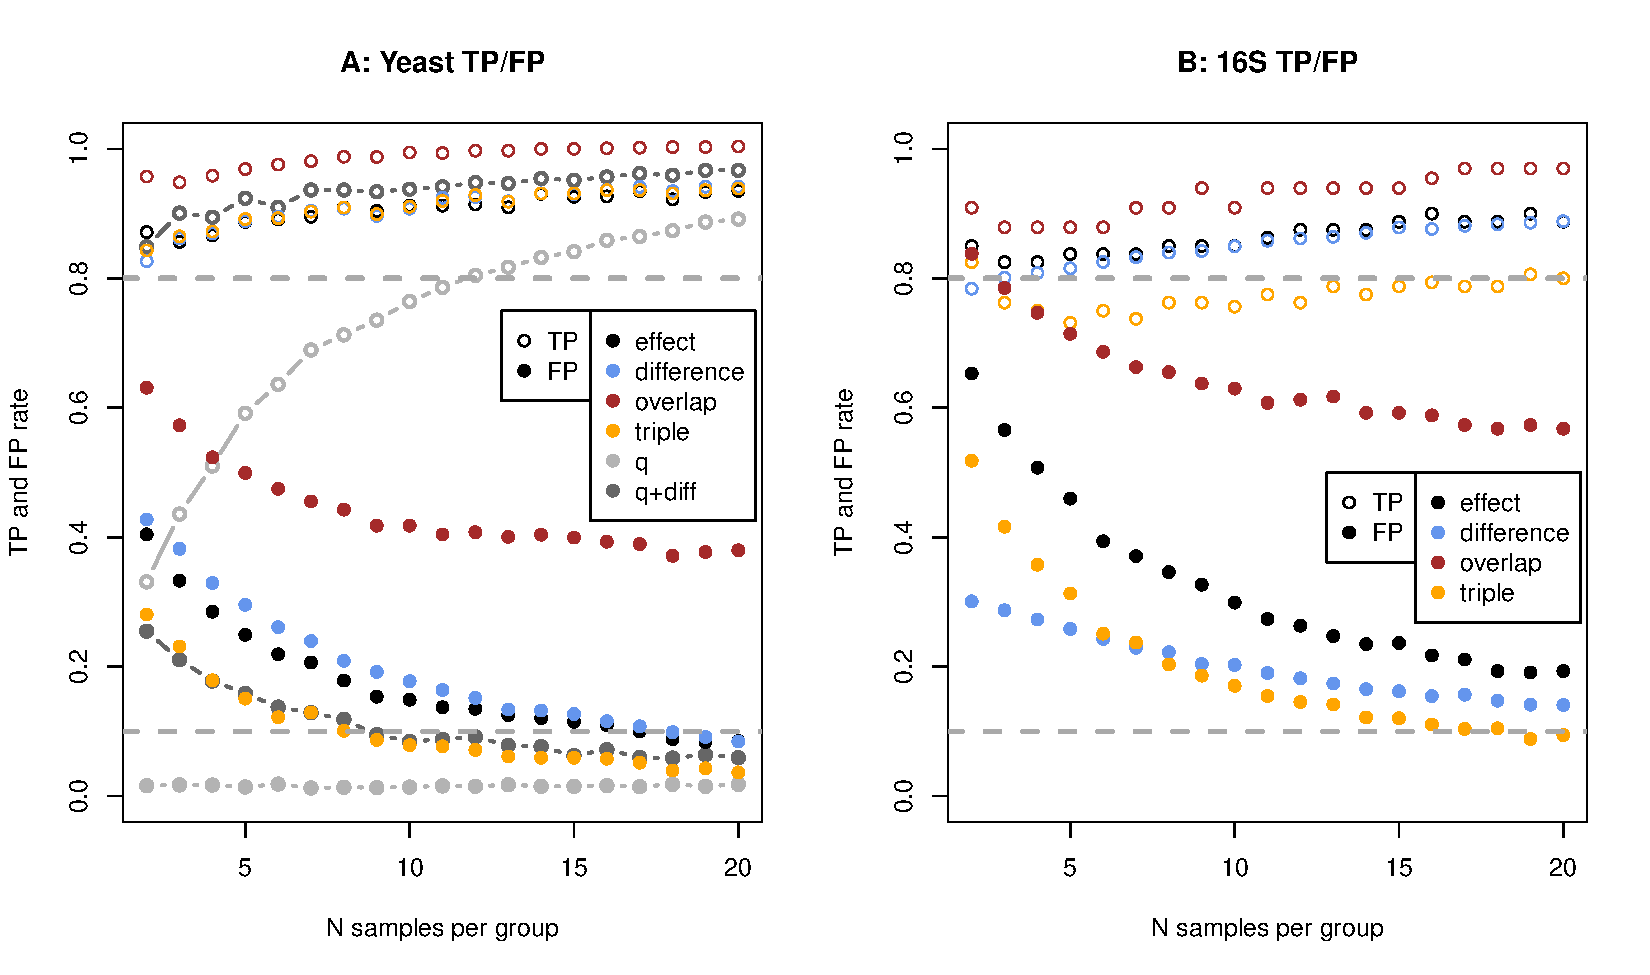
\includegraphics[scale=0.4]{TPvsFP.pdf}}
\caption{True Positive (TP) and False Positive (FP) identifications as a function of per group sample size in the two datasets. The two  panels show the results of randomly sub-sampling the yeast transcriptome and the 16S rRNA gene  datasets 100 times with various numbers of features in each group.  Features that were identified in the subsample and in the full dataset were counted as true positives (TP), and features that were identified in the subsets that were not identified as different in the full dataset were counted as false positives (FP). The panels show the median proportion of TP found by each approach, and the median proportion of all positives that were FP.  Cutoffs used were absolute effect $> 1$, absolute difference $> 1$, overlap of $< 0.1$, or q score of $< 0.1$ (Benjamini-Hochberg adjusted p-value). The triple approach used the intersect of the effect, difference and overlap approaches. 
}
\label{fig:02}
\end{figure}

We examined the relationship between sample size and the number of features identified as significantly different using a null hypothesis testing framework in the yeast dataset. Figure \ref{fig:02}:A shows the median True and False Positive rates. In this analysis we are testing for the ability to detect  features that would have been observed as differentially abundant in the full dataset if we use  a random subset of the data, and the plots show the median value of 100 trials at each sample size. The `q+diff` example in the Proportion panel shows the rate observed for the  Benjamini-Hochberg corrected p-values (q-values) and a 2-fold difference observed when using the edgeR tool (REF), as advised in recent best practices \citep{Schurch:2016aa}. As expected when using p-values alone, we observe that the power of null hypothesis significance test is strongly affected by sample size, and only reaches 90\% power to detect when the per-group sample size is greater than 20. However, the FP rate is effectively 0.  Interestingly, applying both the significance test and the fold-change cutoff caused both the TP and FP rates to increase substantially. At small sample sizes the TP rate its greater than 80\% and the FP rate ranges from $\sim 30$\% and down. Inspection of the results indicated that this was because in this dataset the significance test was all-but irrelevant  since all features with at least a 2-fold change  had a q-score below the threshold of 0.1.   Note that many tools have difficulty estimating the actual FDR in real datasets \citep{Thorsen:2016aa,hawinkel2017}. 

In contrast to q-scores alone, the  TPR  of the $\mathbb{E}$ statistic in the same random datasets is essentially independent of the number of samples for all methods and combinations. However,  the FPR is strongly affected by sample size as was observed for q-scores and difference. Note that even when only two samples are used, the $\mathbb{E}$ statistic identifies over 80\% of the features as different as are identified by the same statistic in the full dataset. Thus, the simple metric outlined here  can correctly identify the `true positive' set even when the number of samples is very small. The tradeoff when using this statistic is that at very low sample sizes the False Discovery Rate (fdr) is extreme; in this dataset and with a cutoff of $\mathbb{E} > 1$, the fdr is 40\% with two samples, but falls to less than 10\% only when there are 15 or more samples. Interestingly, applying a fold-change and an overlap metric (denoted as triple in the figure) cutoff to the $\mathbb{E}$ metric reduces the false discovery rate dramatically, and it is now indistinguishable from the FP rate observed with the q-score and difference combination.  A similar trend is observed with the 16S dataset, where the metrics have extremely good power to detect even at low sample sizes, but have a high false positive rate at low sample sizes. We conclude that the $\mathbb{E}$ measure, alone or in combination with the difference and overlap metric, constitutes a useful and reproducible way to identify differentially abundant features in disparate datasets. 

\section*{Conclusion}

By default, we want to know both `what is significant' and `what is different' \citep{Cui:2003aa}.  Both of these questions can be addressed with a standardized effect size statistic that scales the difference between features by their dispersion. We have found plots of difference and dispersion to be an exceedingly useful tool when examining HTS datasets \citep{gloor:effect}. Furthermore, datasets analyzed by this approach have proven to be remarkably reproducible as shown by independent lab validation \citep{macklaim:2013, nelson:2015vaginal}. 

The $\mathbb{E}$ statistic outlined here is a relatively robust statistic with the attractive property that it consistently  identifies almost all of the true features regardless of the underlying distribution  and the number of samples, as shown in Figure \ref{fig:02}. In marked contrast, even the best p-value based  approaches can identify only a small proportion of the features at small samples sizes that would have been found in the full dataset \citep{Schurch:2016aa}. Thus, the simple metric outlined here  can correctly identify the `true positive' set even when the number of samples is very small. Note that fold-change thresholds, as is commonly used, is not the same as a standardized effect statistic, and applying the threshold values of \citep{Schurch:2016aa} while reducing the features that are found does not necessarily enhance reproducibility. In fact this investigation highlights the danger in relying on fold-change to identify differentially abundant features. We can see that the 16S rRNA gene sequencing datasets have substantially greater numbers of fold-change FP features than does the yeast transcriptome dataset when no difference in expected. This is  because of the substantially greater dispersion observed for the features in the former dataset than in the latter.

The tradeoff when using the $\mathbb{E}$ statistic is that at very low sample sizes the False Discovery Rate can be extreme; in this dataset and with a cutoff of $\mathbb{E} > 1$, the FDR is 40\% with two samples, but falls to less than 10\% only when there are 15 or more samples regardless of dataset. Note that the FDR as measured is assessing congruence with the result in the whole dataset since the actual ground truth is not known. Given that FP are not identified if there is no difference between groups when the sample size is greater than 10 (Figure \ref{fig:fp}:A), it is likely that the FP identified when the groups are different are simply features with lower effect sizes. Supplementary Figure 5 shows that this is in fact the case. Moreover, using the combination of effect, difference and overlap  enhances specificity regardless of dataset. This is because these measures are filtering out different sets of FP features, but identify substantially the same set of TP features: the $\mathbb{E}$ metric is the mid point of the effect size distribution and identifies those features with large standardized change between groups; the overlap metric corresponds to the tail of the $\vec{\mathit{eff}}$ distribution and identifies those features with narrow distributions; the difference between metric identifies those features with large absolute fold change.  

 Further tempering this is the observation that  no false positives are identified when no difference is expected in two different datasets when there are 10 or more samples per group.  Taken together, we suggest that a fold change of at least two, and both $\mathbb{E} > 1$ and overlap $< 0.1$ are robust and reproducible measures that provide an acceptable mix of power and specificity when the sample size is greater than 10 per group in diverse datasets. 

This work  describes the  $\mathbb{E}$ statistic that measures a standardized effect size directly from distributions and not from summary statistics. We show that it is useful when examining high throughput sequencing datasets. The statistic is relatively robust and efficient, and answers the question most desired by the biologist, namely `what is reproducibly different'.   The $\mathbb{E}$ metric is computed in the ALDEx2 R package as the `effect' output where it is the median of the inferred technical and biological data, and in the CodaSeq R package where it acts only on the point estimates of the data. Interactive exploration of effect sizes can be done in the omicplotR Bioconductor package \citep{omicplot}.

\section*{Acknowledgements}

We thank past and present members of the lab for helpful comments and insights. In particular Dan Giguere suggested the title, and Brandon Lieng developed the code in ALDEx2 that provided Figure 1.

\vspace{-12pt}
\section*{Funding}

This work was funded by NSERC (RGPIN-03878-2015) awarded to G.B.G.\vspace*{-12pt}

\begin{thebibliography}{}

\bibitem[Aitchison, 1986]{aitchison:1986}
Aitchison, J. (1986).
\newblock {\em The Statistical Analysis of Compositional Data}.
\newblock Chapman \& Hall.

\bibitem[Bian et~al., 2017]{bian:2017}
Bian, G., Gloor, G.~B., Gong, A., Jia, C., Zhang, W., Hu, J., Zhang, H., Zhang,
  Y., Zhou, Z., Zhang, J., Burton, J.~P., Reid, G., Xiao, Y., Zeng, Q., Yang,
  K., and Li, J. (2017).
\newblock The gut microbiota of healthy aged Chinese is similar to that of the
  healthy young.
\newblock {\em mSphere}, 2(5):e00327--17.

\bibitem[Coe, 2002]{coe2002s}
Coe, R. (2002).
\newblock It's the effect size, stupid: What effect size is and why it is
  important.

\bibitem[Colquhoun, 2014]{Colquhoun:2014aa}
Colquhoun, D. (2014).
\newblock An investigation of the false discovery rate and the
  misinterpretation of p-values.
\newblock {\em R Soc Open Sci}, 1(3):140216.

\bibitem[Cui and Churchill, 2003]{Cui:2003aa}
Cui, X. and Churchill, G.~A. (2003).
\newblock Statistical tests for differential expression in cDNA microarray
  experiments.
\newblock {\em Genome Biol}, 4(4):210.1 -- 210.10.

\bibitem[Cumming, 2008]{Cumming:2008aa}
Cumming, G. (2008).
\newblock Replication and p intervals: p values predict the future only
  vaguely, but confidence intervals do much better.
\newblock {\em Perspect Psychol Sci}, 3(4):286--300.

\bibitem[Fernandes et~al., 2013]{fernandes:2013}
Fernandes, A.~D., Macklaim, J.~M., Linn, T.~G., Reid, G., and Gloor, G.~B.
  (2013).
\newblock Anova-like differential expression (ALDEX) analysis for mixed
  population RNA-seq.
\newblock {\em PLoS One}, 8(7):e67019.

\bibitem[Fernandes et~al., 2014]{fernandes:2014}
Fernandes, A.~D., Reid, J.~N., Macklaim, J.~M., McMurrough, T.~A., Edgell,
  D.~R., and Gloor, G.~B. (2014).
\newblock Unifying the analysis of high-throughput sequencing datasets:
  characterizing {RNA}-seq, 16{S} r{RNA} gene sequencing and selective growth
  experiments by compositional data analysis.
\newblock {\em Microbiome}, 2:15.1--15.13.

\bibitem[Giguere et~al., 2019]{omicplot}
Giguere, D., Macklaim, J., and Gloor, G. (2019).
\newblock omicplotR: Visual exploration of omic datasets using a shiny app.
\newblock Bioconductor v1.4.0.

\bibitem[Gloor et~al., 2016a]{gloor:effect}
Gloor, G.~B., Macklaim, J.~M., and Fernandes, A.~D. (2016a).
\newblock Displaying variation in large datasets: Plotting a visual summary of
  effect sizes.
\newblock {\em Journal of Computational and Graphical Statistics},
  25(3C):971--979.

\bibitem[Gloor et~al., 2017]{gloorFrontiers:2017}
Gloor, G.~B., Macklaim, J.~M., Pawlowsky-Glahn, V., and Egozcue, J.~J. (2017).
\newblock Microbiome datasets are compositional: And this is not optional.
\newblock {\em Front Microbiol}, 8:2224.

\bibitem[Gloor et~al., 2016b]{gloorAJS:2016}
Gloor, G.~B., Macklaim, J.~M., Vu, M., and Fernandes, A.~D. (2016b).
\newblock Compositional uncertainty should not be ignored in high-throughput
  sequencing data analysis.
\newblock {\em Austrian Journal of Statistics}, 45:73--87.

\bibitem[Halsey et~al., 2015]{Halsey:2015aa}
Halsey, L.~G., Curran-Everett, D., Vowler, S.~L., and Drummond, G.~B. (2015).
\newblock The fickle p value generates irreproducible results.
\newblock {\em Nat Methods}, 12(3):179--85.

\bibitem[Hawinkel et~al., 2018]{hawinkel2017}
Hawinkel, S., Mattiello, F., Bijnens, L., and Thas, O. (2018).
\newblock A broken promise : microbiome differential abundance methods do not
  control the false discovery rate.
\newblock {\em BRIEFINGS IN BIOINFORMATICS}.

\bibitem[Ioannidis, 2005]{Ioannidis:2005aa}
Ioannidis, J. P.~A. (2005).
\newblock Why most published research findings are false.
\newblock {\em PLoS Med}, 2(8):e124.

\bibitem[Kaul et~al., 2017]{Kaul:2017aa}
Kaul, A., Mandal, S., Davidov, O., and Peddada, S.~D. (2017).
\newblock Analysis of microbiome data in the presence of excess zeros.
\newblock {\em Front Microbiol}, 8:2114.

\bibitem[Lovell et~al., 2015]{Lovell:2015}
Lovell, D., Pawlowsky-Glahn, V., Egozcue, J.~J., Marguerat, S., and B{\"a}hler,
  J. (2015).
\newblock Proportionality: a valid alternative to correlation for relative
  data.
\newblock {\em PLoS Comput Biol}, 11(3):e1004075.

\bibitem[Lovell et~al., 2020]{lovell2020counts}
Lovell, D.~R., Chua, X.-Y., and McGrath, A. (2020).
\newblock Counts: an outstanding challenge for log-ratio analysis of
  compositional data in the molecular biosciences.
\newblock {\em NAR Genomics and Bioinformatics}, 2(2):lqaa040.

\bibitem[Macklaim et~al., 2013]{macklaim:2013}
Macklaim, J.~M., Fernandes, A.~D., Di~Bella, J.~M., Hammond, J.-A., Reid, G.,
  and Gloor, G.~B. (2013).
\newblock Comparative meta-{RNA}-seq of the vaginal microbiota and differential
  expression by \em{Lactobacillus iners} in health and dysbiosis.
\newblock {\em Microbiome}, 1(1):12.

\bibitem[Marioni et~al., 2008]{Marioni:2008}
Marioni, J.~C., Mason, C.~E., Mane, S.~M., Stephens, M., and Gilad, Y. (2008).
\newblock {RNA-seq}: an assessment of technical reproducibility and comparison
  with gene expression arrays.
\newblock {\em Genome Res}, 18(9):1509--17.

\bibitem[Nakagawa, 2004]{shinichi:2004}
Nakagawa, S. (2004).
\newblock A farewell to Bonferroni: the problems of low statistical power and
  publication bias.
\newblock {\em Behavioral Ecology}, 15(6):1044--1045.

\bibitem[Nelson et~al., 2015]{nelson:2015vaginal}
Nelson, T.~M., Borgogna, J.-L.~C., Brotman, R.~M., Ravel, J., Walk, S.~T., and
  Yeoman, C.~J. (2015).
\newblock Vaginal biogenic amines: biomarkers of bacterial vaginosis or
  precursors to vaginal dysbiosis?
\newblock {\em Frontiers in physiology}, 6.

\bibitem[Quinn et~al., 2019]{Quinn:2019aa}
Quinn, T.~P., Erb, I., Gloor, G., Notredame, C., Richardson, M.~F., and
  Crowley, T.~M. (2019).
\newblock A field guide for the compositional analysis of any-omics data.
\newblock {\em Gigascience}, 8(9).

\bibitem[Schurch et~al., 2016]{Schurch:2016aa}
Schurch, N.~J., Schofield, P., Gierli{\'n}ski, M., Cole, C., Sherstnev, A.,
  Singh, V., Wrobel, N., Gharbi, K., Simpson, G.~G., Owen-Hughes, T., Blaxter,
  M., and Barton, G.~J. (2016).
\newblock How many biological replicates are needed in an RNA-seq experiment
  and which differential expression tool should you use?
\newblock {\em RNA}, 22(6):839--51.

\bibitem[Soneson and Delorenzi, 2013]{Soneson:2013}
Soneson, C. and Delorenzi, M. (2013).
\newblock A comparison of methods for differential expression analysis of
  {RNA-seq} data.
\newblock {\em BMC Bioinformatics}, 14:91.

\bibitem[Thorsen et~al., 2016]{Thorsen:2016aa}
Thorsen, J., Brejnrod, A., Mortensen, M., Rasmussen, M.~A., Stokholm, J.,
  Al-Soud, W.~A., S{\o}rensen, S., Bisgaard, H., and Waage, J. (2016).
\newblock Large-scale benchmarking reveals false discoveries and count
  transformation sensitivity in 16{S} r{RNA} gene amplicon data analysis
  methods used in microbiome studies.
\newblock {\em Microbiome}, 4(1):62.

\bibitem[Tsilimigras and Fodor, 2016]{Tsilimigras:2016aa}
Tsilimigras, M. C.~B. and Fodor, A.~A. (2016).
\newblock Compositional data analysis of the microbiome: fundamentals, tools,
  and challenges.
\newblock {\em Ann Epidemiol}, 26(5):330--5.

\bibitem[Weiss et~al., 2017]{Weiss:2017aa}
Weiss, S., Xu, Z.~Z., Peddada, S., Amir, A., Bittinger, K., Gonzalez, A.,
  Lozupone, C., Zaneveld, J.~R., V{\'a}zquez-Baeza, Y., Birmingham, A., Hyde,
  E.~R., and Knight, R. (2017).
\newblock Normalization and microbial differential abundance strategies depend
  upon data characteristics.
\newblock {\em Microbiome}, 5(1):27.
\end{thebibliography}

\end{document}
